\documentclass[a4paper,12pt]{report}
\usepackage{graphicx}
\usepackage{titlesec}
\titleformat{\chapter}{}{}{0em}{\bf\LARGE}
\usepackage[utf8]{inputenc}
% Title Page
\title{Middle East Technical University\\Department of Physics\\PHYS222 Optics and Waves Laboratory\\\textbf{Experiment OW-11 Spectral Energy Distribution In Different Filters\\Laboratory Report}}

\author{Oğuzhan ÖZCAN\\1852334\\\\Partner: İnci SAİM\\\\Teaching Assistant: Kamil ÇINAR}


\begin{document}
\maketitle
\tableofcontents
\listoffigures
\listoftables
\chapter{Theory}
An instrument used to view spectra by eye is called a \textit{spectroscope}, while
one employed with any sort of electronic detector is called a \textit{spectrometer}. A spectrometer has relatively poor resolving power compared to a Fabry-Perot
interferometer. Nevertheless, a spectrometer is not hampered by the serious
limitation imposed by free spectral range. A spectrometer is able to measure a
wide range of wavelengths simultaneously [1]. An important application of this technique is to astronomy. As light generated
within the sun passes through the sun’s atmosphere, certain wavelengths are
selectively absorbed. The result is that the spectrum of sunlight produced by a
diffraction grating has dark absorption lines [2]. The first assumption in spectroscopic measurements is that Beer's law
relationship applies between a change in spectrometer response and the
concentration of analyte material present in a sample specimen. The
\textit{Bouguer, Lambert,} and \textit{Beer} relationship assumes that the transmission of a
sample within an incident beam is equivalent to 10 exponent the negative
product of the molar extinction coefficient (in L$\cdot$mol$^{-1}$cm$^{-1}$), multiplied
by the concentration of a molecule in solution (in mol $\cdot$ L$^{-1}$) times the pathlength
(in cm) of the sample in solution. For more precise definition of spectrometry we must give some attention to transmittance, reflectance and absorbtance.\\\\
Let consider a circular beam of light incident on a surface and there is a illuminated spot of area A. Since light beam can act as a wave, we should give a Poynting vector
\begin{center}
	$\vec{S}=c^{2}\epsilon_{0}\vec{E}\times\vec{B}$
\end{center}
then we can define radiant flux density or irradiance in W/m$^{2}$
\begin{center}
	$I=\frac{c\epsilon_{0}}{2}E_{0}^{2}$
\end{center}
Note that the this is the average energy per unit time which is crossing per unit area. In this case let $I_{i}$, $I_{r}$ and $I_{t}$ be the incident, reflected and transmitted irradiances. Now we can define \textit{reflectance} $R$,
\begin{center}
	{\large $R=\frac{I_{r}A\cos\theta_{r}}{I_{i}A\cos\theta_{i}}=\frac{I_{r}}{I_{i}}$}
\end{center}
In the same way, the transmittance $T$ is defined as ratio of the transmitted to the incident flux and $T$ can defined as 
\begin{center}
	{\large $T=\frac{I_{t}\cos\theta_{t}}{I_{i}\cos\theta_{i}}$}
\end{center}
When there is no absorption we can say thar \textit{R+T=1} [3]. At this point we have to define \textit{Beer's law.} According to Beer's law, The imaginary part of the refractive index corresponds to attenuation, or possibly
amplification, of the wave during propagation. It is convenient to define
a complex wave vector:
\begin{center}
$k=k'-$j$k'' with \mid k'\mid=n'$$\omega$/c and $\mid$ k''$\mid$=n''$\omega$/c 
\end{center} 	
\begin{center}
	$E=E_{0} e^{j\omega(t-z/c)}$
\end{center}
where $e^{j\omega(t-z/c)}$ is a complex number that keeps a constant modulus during the propagation. Then we can define intensity as 
\begin{center}
	$I=I_{0}e^{-2k''z}=I_{0}e^{-\alpha z}$ where $\alpha=2k''$
\end{center}
This relationship called as Beer's law and $\alpha$ is correspond to \textit{absoption coefficient} [4]. We can describe transmittance and absorption coefficient more simply by following equaitons
\begin{center}
	{\large $T=\frac{I}{I_{0}}$}
\end{center}
where $I_{0}$ is the intensity of incident energy and $I$ is the intensity of transmitted light. Now we can determine the absorptance as follows 
\begin{center}
	$A=-\log(\frac{I}{I_{0}})=-\log T$
\end{center} 
The following statements are true for Beer's law:\\
1	The relationship between transmittance and concentration is non-linear\\2	The relationship between absorbance and concentration is linear [4].\\\\
There are different types of spectrometers such as discrete photometers, single beam, double beam, interferometer based and emission spectrometers. Single beam spectrometer have a single optical channel which is configured to measure either sample of reference channel but not both simultaneously.\\\\
Another important quantity about spectrometer is filters. Two basic types of interference filters exist: bandpass filters and edge filters.
Bandpass filters transmit light only for a defined spectral band. The transmitted
spectral bands may be from less than 1 nm full bandwidth at half
maximum (FWHM) transmission band height to 50 nm or more FWHM.
Edge filters transmit light either above or below a certain wavelength
region; these are referred to as "cut-on" or "cut-off" types, respectively.
These filters transmit efficiently throughout a broad region until the transmission
limit of the filter substrate material is reached.
Interference filters consist of a solid Fabry-Perot cavity. This is a device
made of a sandwich of two partially reflective metallic layers separated by a
transparent dielectric spacer layer. The partially reflective layers are made
of higher refractive index than the dielectric spacer layer and are 2/4 in
thickness, where 2 is the peak wavelength (wavelength of maximum
transmission) for the filter. The lower refractive index spacer layer is made
to 2/2 thickness. The thickness of the dielectric spacer layer determines the
actual peak transmission wavelength for the filter. Only the 2/2 light transmits
with high efficiency; the other wavelengths experience constructive
interference between the multiple-order reflections from the two partially
reflective layers. The wavelength position of the transmittance peak ($\lambda_{t}$) through either a
Fabry-Perot interferometer or bandpass interference filter is given as
\begin{center}
	{\Large $\lambda_{t}=\frac{2\times n_{\sigma}t_{\sigma}\cos\alpha}{n}$}
\end{center}
where $\lambda_{t}$ is the wavelength of maximum transmittance for the filter, $n_{\sigma}$ is the refractive index of the dielectric spacer, $t_{\sigma}$ is the thickness of the dielectric
spacer in micrometers, $\alpha$ is the angle of incidence of the light impinging
onto the dielectric spacer, and $n$ is the order number for the interference (n
nonzero integer as 0, 1, 2...).




























\chapter{Data and Results}
\begin{table}[h]
	\begin{center}
\begin{tabular}{|c|c|c|c|}
	\hline Filter & $\lambda_{cut-on}$ & $\lambda_{int}$ & $\lambda_{max}$ \\ 
	\hline Red & 618 nm & 704 nm & - \\ 
	\hline Green & 837 nm & 896 nm & 525 nm \\ 
	\hline Blue & 700 nm & 770 nm & 455 nm \\ 
	\hline 
\end{tabular}  
\end{center}
\caption{$\lambda_{cut-on}$, $\lambda_{int}$, $\lambda_{max}$ wavelengths for filters} 
\end{table}
\textbf{1. Plot Transmission Spectrum (\textit{T} vs $\lambda$) for each filters and obtain $\lambda_{cut-on}$, $\lambda_{int}$, $\lambda_{max}$.} 
\begin{figure}[h!]
\centering
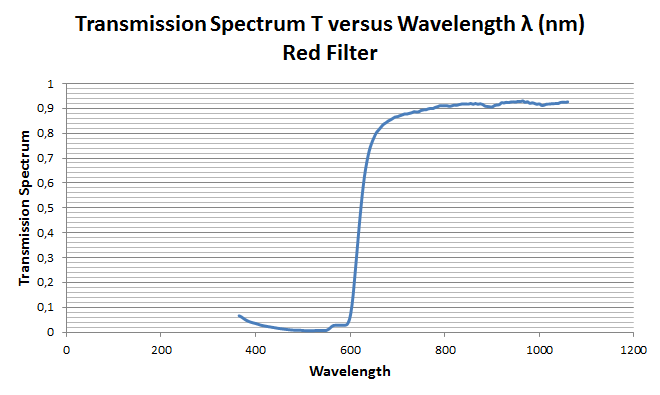
\includegraphics[width=1.0\linewidth, height=0.4\textheight]{Red}
\caption{Transmission Spectrum vs Wavelength Graph for Red Filter}
\label{fig:Red}
\end{figure}
\begin{figure}[h!]
\centering
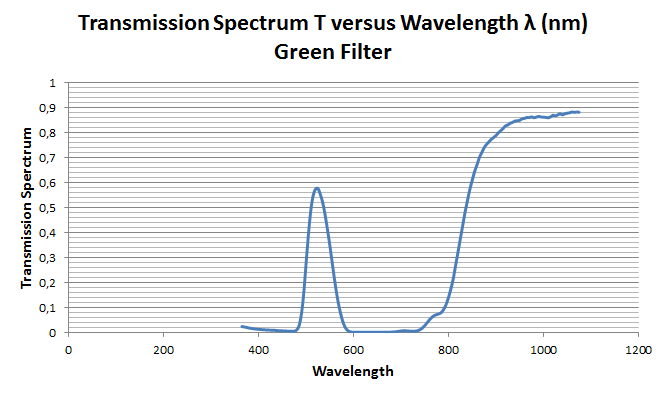
\includegraphics[width=1.0\linewidth, height=0.4\textheight]{Green}
\caption{Transmission Spectrum vs Wavelength Graph for Green Filter}
\label{fig:Green}
\end{figure}
\begin{figure}[h!]
\centering
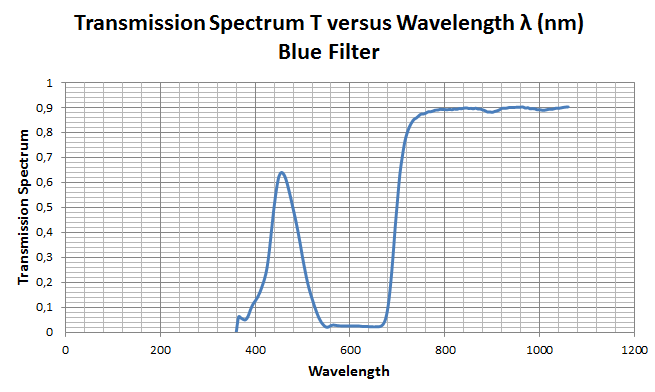
\includegraphics[width=1.0\linewidth, height=0.4\textheight]{Blue}
\caption{Transmission Spectrum vs Wavelength Graph for Blue Filter}
\label{fig:Blue}
\end{figure}

\textbf{2. Plot Absorption Spectrum (\textit{A} vs $\lambda$) for each filter.}\\\\

\begin{figure}[h!]
\centering
\includegraphics[width=1.0\linewidth, height=0.4\textheight]{"Abs Red"}
\caption{Absorption Spectrum vs Wavelength Graph for Red Filter}
\label{fig:AbsRed}
\end{figure}

\begin{figure}[h!]
\centering
\includegraphics[width=1.0\linewidth, height=0.4\textheight]{"Abs Green"}
\caption{Absorption Spectrum vs Wavelength Graph for Green Filter}
\label{fig:AbsGreen}
\end{figure}

\begin{figure}[h!]
\centering
\includegraphics[width=1.0\linewidth, height=0.4\textheight]{"Abs Blue"}
\caption{Absorption Spectrum vs Wavelength Graph for Blue Filter}
\label{fig:AbsBlue}
\end{figure}
\textbf{3. Identify which filters are longpass and bandpass by examining your graphs.}\\
When we look at graphs we can observe that following results. Red filter is behave as a longpass filter, blue and green filters are behave as both bandpass and longpass filter.\\\\
\textbf{4. By using the transmittance and absorbance values do you think there is any reflection? Explain briefly how do you decide for this?}\\
Yes there is a reflection in our results. We can obtain this result by using definition of energy distribution. Summation of transmittance, absorbance and reflectence must equal to 1. By using following calculations we can observe reflectence with related wavelengths. In these calculations I am going denote transmittance as T, absorbance as A and reflectance as R. Thus T+A+R=1\\
For Red Filter at 700 nm wavelength:\\
$T_{Red}=0.8669$  and  $A_{Red}=0.062031$ so $R_{Red}=0.071069$\\
For Green Filter at 800 nm wavelength:\\
$T_{Green}=0.1403$  and  $A_{Green}=0.852942$ so $R_{Green}=0.00675$\\
For Blue Filter at 700 nm wavelength:\\
$T_{Blue}=0.5264$  and  $A_{Blue}=0.278684$ so $R_{Blue}=0.194916$\\
























\chapter{Discussion and Conclusion}
\textbf{1.What are the possible errors in the experiment?}\\
In this experiment we used a spectrometer device and brand of spectrometer is \textit{Jenway 6400.} Since we did not make any calculation or experiment, we do not have a possible error. However, according to manufacturer this spectrometer has an accuracy $\pm$1.0 nm [5].\\\\
\textbf{2.What kind of approximation did you take into consideration while you were obtaining the physical quantities and how do they affect your results?}\\
Only approximations was taken when calculating $\lambda_{cut-on}$, $\lambda_{int}$ and $\lambda_{max}$ values.\\\\
\textbf{3.What discrepancies did you encounter between the calculated quantities and theoretical or literature values?}\\
As we know transmittance cannot exceed 1. This is why I thought that absorption also cannot exceed 1. However in our results Absorption spectrum is higher than 1 in some wavelengths. As I seen in some articles when absorption is higher than 1.5, then absorption values are not useful for experimental calculations. Besides, \textit{Jenway 6400} has a range of absorptance from -0.300 A to 3.000 A. Also I thought that plotting a graph of absorption spectrum which does not include an absorption that is higher than 1 would be useful to understand the behaviour of filters (See Figures 3.1, 3.2, 3.3). As seen in the graphs when we do not take data above 1, graphs are very familiar with transmission graphs.\\\\
\begin{figure}[h!]
\centering
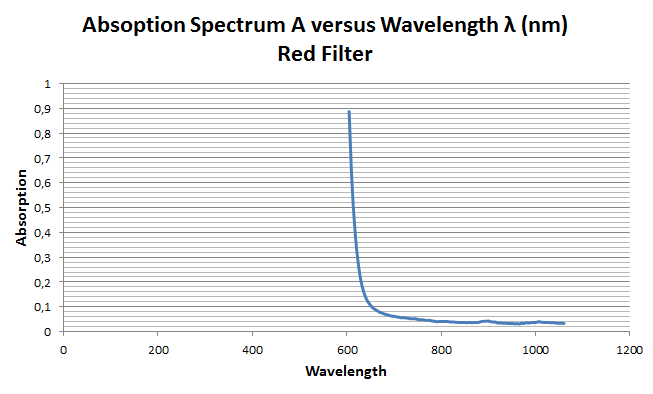
\includegraphics[width=1.0\linewidth, height=0.4\textheight]{A-Red}
\caption{Absorption $\leq$ 1 for Red Filter}
\label{fig:A-Red}
\end{figure}
\begin{figure}[h!]
\centering
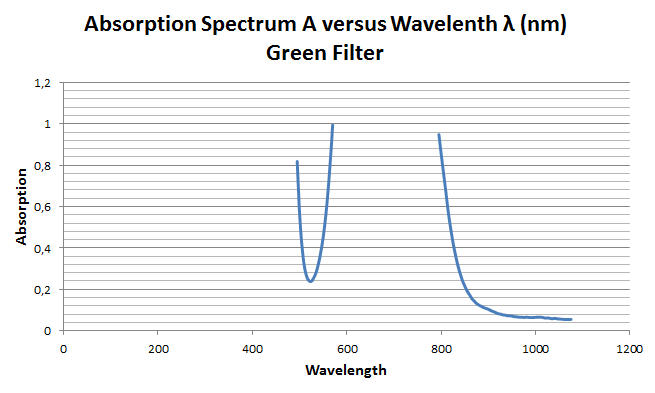
\includegraphics[width=1.0\linewidth, height=0.4\textheight]{A-Green}
\caption{Absorption $\leq$ 1 for Green Filter}
\label{fig:A-Green}
\end{figure}
\begin{figure}[h!]
\centering
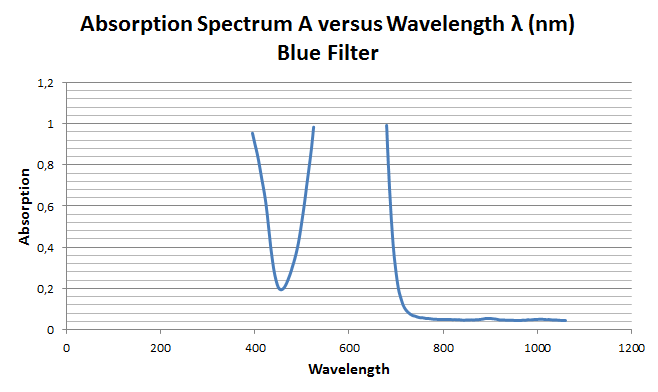
\includegraphics[width=1.0\linewidth, height=0.4\textheight]{A-Blue}
\caption{Absorption $\leq$ 1 for Blue Filter}
\label{fig:A-Blue}
\end{figure}
\textbf{4.What is your overall conclusion?}\\
In my opinion observation of spectrometer was succesful. We examine the behaviours different filters. Theoretical and experimental values are very close to each other.  























\chapter{Application}
\textbf{Colorimetry}\\
Colorimetry is the science of the measurement of colours. It involves the replacement of subjective responses, such as "light blue", "rich dark purple", "bright gold", with an objective numerical system. This study began with the work of Young, Helmholtz and Maxwell in the early 19th century, who recognized the principles of additive and subtractive colour mixing, and proposed the trichromatic nature of human colour vision. The science began to be formalized in 1931, when the Commission International de l'Eclairage (CIE) recommended a system of colour specification based on the three tristimulus values X, Y and Z.\\\\
Three things contribute to our perception of the colour of an object: the nature of the illumination, the optical properties of the object itself and the response of the human eye. The nature of the illumination can be characterized by the spectral power distribution $S(\lambda)$ of the light source, the relative intensity of the illumination at each wavelength in the visible spectrum. The object reflects a certain fraction of the incident light and this can be characterized by the reflactance spectrum $R(\lambda)$. The intensity of light entering the eye, $I(\lambda)$, is the product of these terms. Thus in order to measure colour, and to specify colour by numbers, it is necessary to specify each of these three components of the colour trio. In 1931, the CIE recommended standard illuminants for use in colorimetry, published data representing the standard observer and recommended standard optical geometries for use in colour-measuring instruments.\\\\
The RGB (Red, Green, Blue) system of colour specification was based on the trichromatic theory of colour vision and the colour-matching experiments carried out by Guild and Wright. It had been suggested by Maxwell in 1860  that if the specifications of the red, green and blue lamps used in such experiments were known, then the amounts of each light required to match a sample colour would provide a numerical specification of that colour.\\\\
On the other hand, the XYZ systen of colour specification was closely based on the RGB system. The difference lies in the fact that R, G and B were real light sources of known specifications. X, Y and Z are theoretical sources which are more saturated than any real light source, and allow matching of any real colour using positive amounts of the three primary sources. Note that XYZ values may be calculated from reflactance values using similar equaitons to those for RGB [6].
\chapter{References}
$[1]$ Peatross, J., \& Ware, M. (2014). \textit{Physics of Light and Optics} (2013 ed., p. 285). Provo, UT: Brigham Young University Press.\\
$[2]$ Young, H. (2012). \textit{University Physics with Modern Physics: Sears and Zemansky's} (13th ed., p. 1203). Boston: Pearson education.\\
$[3]$ Hecht, E. (2002). \textit{Optics} (4th ed., p. 120). Reading, Mass.: Addison-Wesley.\\
$[4]$ Drude, P., Mann, C., \& Millikan, R. (1959). \textit{The Theory of Optics} (1st ed., p. 365). New York, NY: Dover Publications.\\
$[5]$ 6400 and 6405 Scanning Spectrophotometers. (n.d.). Retrieved April 26, 2015, from http://www.jenway.com/adminimages/Page-72-6400-6405.pdf\\
$[6]$ Gilchrist, A., \& Nobbs, J. (2000). Colorimetry. In J. Lindon, G. Tranter, \& J. Holmes (Eds.), \textit{Encyclopedia of Spectroscopy And Spectrometry} (1st ed., Vol. 1, p. 337). San Diego: Academic Press.



























































































\end{document}          
